%Master File:lectures.tex

\lesson{Use Data Structures and Algorithms!}
\vspace*{-1cm}
\begin{center}
  \includegraphics[height=10cm]{suffix_tree}
\end{center}
\keywords{Course structure, examples of data structures and algorithms}

%%%%%%%%%%%%%%%%%%%%%%% Next Slide %%%%%%%%%%%%%%%%%%%%%%%

\renewcommand{\Outline}{%
\begin{slide}
\section{Outline}
\begin{minipage}{10cm}
  \vfill
  \begin{enumerate}
    \outlineitem{Course structure}{intro}
    \outlineitem{Example of Using DSA}{examplesjhds}
    \outlineitem{Sophisticated Program}{big}
    \outlineitem{State-of-the-Art}{bbig}
  \end{enumerate}
  \vfill
\end{minipage}\hfill
\begin{minipage}{12cm}
  \includegraphics[width=12cm]{suffix_tree}
\end{minipage}
\end{slide}
\addtocounter{outlineitem}{1}
}

\setcounter{outlineitem}{1}
\Outline
\toptarget{firstoutline}

%%%%%%%%%%%%%%%%%%%%%%% Next Slide %%%%%%%%%%%%%%%%%%%%%%%

\begin{slide}
\section{Welcome to Algorithms and Analysis}
  
\begin{PauseHighLight}
  \begin{itemize}
  \item Taught by Dr Daniela Mihai and me (Adam Pr\"ugel-Bennett)\pause
  \item I'm teaching you algorithms\pause{} and data
    structures\pauseb{} in C++\pauseb
  \item The analysis is an ability to reason about programming\pause
  \item Learning C++ will be a joint effort involving
    \textit{Low-level programming}, me\pause{} and you\pauseb
  \item My ambition is not only to teach you data structures and
    algorithms academically\pause, but also to get to a new level of
    coding\pauseb
  \end{itemize}
\end{PauseHighLight}

\end{slide}

%%%%%%%%%%%%%%%%%%%%%%% Next Slide %%%%%%%%%%%%%%%%%%%%%%%

\begin{slide}
\section{Course Structure}

\begin{PauseHighLight}
  \begin{itemize}
  \item 30ish lectures\pause
  \item 4 labs (worth 10\%)\pauseb
  \item 1 coursework (worth 30\%)\pauseb
  \item Week 6 is a reading week with an in-class exam (worth 10\%?)\pauseb
  \item Final exam (worth 50\%?)\pauseb
  \end{itemize}
\end{PauseHighLight}


\end{slide}



%%%%%%%%%%%%%%%%%%%%%%% Next Slide %%%%%%%%%%%%%%%%%%%%%%%

\begin{slide}
\section{Recommended Course Text}

\begin{minipage}{10cm}
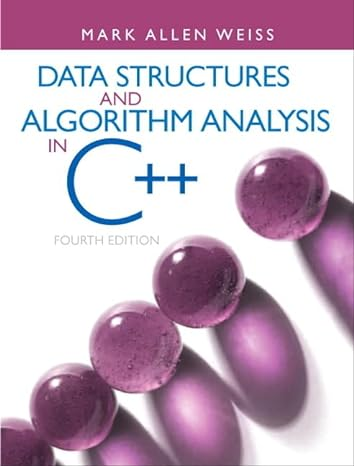
\includegraphics[width=10cm]{weiss}
\end{minipage}\hfill
\begin{minipage}{12cm}
  \begin{PauseHighLight}
    \begin{itemize}
    \item \textit{Data Structures and Algorithm Analysis in C++} by
      M.~A.~Weiss\pause
      \begin{itemize}
      \item Best introduction to Data Structures and Algorithms\pause
      \item Not huge, but covers all the basics\pause
      \end{itemize}
    \item Available in the library\pause
    \end{itemize}
  \end{PauseHighLight}
\end{minipage}

\end{slide}


%%%%%%%%%%%%%%%%%%%%%%% Next Slide %%%%%%%%%%%%%%%%%%%%%%%

\begin{slide}
\section{What is a Data Structure?}

\begin{PauseHighLight}
  \begin{quote}\it
    any of various methods of organising data items (as records) in a computer
  \end{quote}\pause
  \begin{itemize}
  \item Container for data\pause
  \item E.g. sets, stacks, lists, trees, graphs\pause
  \item Clean interface, e.g. \texttt{push}, \texttt{pop},
    \texttt{delete}\pause
  \item Usually designed for fast or convenient access \pause
\end{itemize}
\end{PauseHighLight}
\end{slide}


%%%%%%%%%%%%%%%%%%%%%%% Next Slide %%%%%%%%%%%%%%%%%%%%%%%

\begin{slide}
\section{What is an Algorithm?}

\begin{PauseHighLight}
  \begin{quote}\it
    a sequence of unambiguous instructions for solving a problem,
    i.e. for obtaining a required output for a legitimate input in a
    finite amount of time
  \end{quote}\pause
  \begin{itemize}
  \item E.g. \texttt{sort, search, match}\pause
  \item Well defined and generic\pause
  \item Guarantees on performance\pause
  \end{itemize}
\end{PauseHighLight}
\end{slide}

%%%%%%%%%%%%%%%%%%%%%%% Next Slide %%%%%%%%%%%%%%%%%%%%%%%

\begin{slide}
\section[-1]{Exemplary OO-Software}

\begin{PauseHighLight}
  \begin{itemize}
  \item Abstraction from details of problem\pause
  \item Declaration of intention\pause
  \item Clean interfaces\pause
  \item Hidden implementations\pause
  \item Makes programs readable and maintainable\pause
  \item Reuse code\pause---don't even have to write it yourself\pause
    \begin{quote}
      \textit{Thou shall not re-implement common data structures}\pauseb
    \end{quote}
  \end{itemize}
\end{PauseHighLight}
\end{slide}

%%%%%%%%%%%%%%%%%%%%%%% Next Slide %%%%%%%%%%%%%%%%%%%%%%%
\Outline

%%%%%%%%%%%%%%%%%%%%%%% Next Slide %%%%%%%%%%%%%%%%%%%%%%%

\begin{slide}
\section{Example: Sort program}

\begin{PauseHighLight}
  \begin{itemize}
  \item Suppose we want to write a program to
    \begin{itemize}
    \item read an input file of integers
    \item sort the integers
    \item write a list of integers to standard out
    \end{itemize}\pause
  \item In Unix there is a command called \texttt{sort} which does just
    this\pause
  \item Note that you don't know the number of inputs
  \end{itemize}\pause
\end{PauseHighLight}

\end{slide}

%%%%%%%%%%%%%%%%%%%%%%% Next Slide %%%%%%%%%%%%%%%%%%%%%%%


\begin{slide}
\section{Code for sort}
\pausebuild

\vspace*{-1cm}
\begin{cpp}
#include <iostream>
#include <fstream>

int main(int argc, char** argv) {
  std::ifstream myfile(argv[1]); 

  int array_size = 10;
  int* array = new int[array_size];
  int cnt = 0;
  while(myfile.good()) {
    if (cnt==array_size) {
      int* new_array = new int[2*array_size];
      for(int i=0; i<array_size; ++i)
	new_array[i] = array[i];
      delete[] array;
      array = new_array;
      array_size *= 2;
    }
    myfile >> array[cnt++];
  }



  
  for(int i=0; i<cnt; ++i) {
    int index = 0;
    for(int j=1; j<cnt-i; ++j) {
      if (array[j]<array[index])
	index = j;
    }
    std::cout << array[index] << std::endl;
    array[index] = array[cnt-i-1];
  }
}

\end{cpp}
\vspace*{-1cm}\pause\vspace{-0.5cm}
\end{slide}

%%%%%%%%%%%%%%%%%%%%%%% Next Slide %%%%%%%%%%%%%%%%%%%%%%%

\begin{slide}
\section{Notes on Code}

\begin{PauseHighLight}
  \begin{itemize}
  \item Details of code don't matter\pause
  \item Simple program ($\sim20$ lines of code)\pause
  \item Uses a simple array\pause
  \item Difficult to see what is going on\pause
  \item On 100\,000 inputs it takes 10 seconds to run\pause
  \end{itemize}
\end{PauseHighLight}

\end{slide}



%%%%%%%%%%%%%%%%%%%%%%% Next Slide %%%%%%%%%%%%%%%%%%%%%%%

\begin{slide}
\section{Using Data Structures and algorithms}
\pausebuild
\begin{cpp}
#include <iostream>
#include <fstream>
#include <iterator>
#include <vector>
#include <algorithm>
using namespace std;

int main(int argc, char *argv[])
{
  ifstream in(argv[1]);
  vector<int> data;
  copy(istream_iterator<int>(in), istream_iterator<int>(), 
       back_inserter(data));
  sort(data.begin(), data.end());
  copy(data.begin(), data.end(), ostream_iterator<int>(cout,"\n"));
}
\end{cpp}\pause\vspace{-0.5cm}
\end{slide}

%%%%%%%%%%%%%%%%%%%%%%% Next Slide %%%%%%%%%%%%%%%%%%%%%%%

\begin{slide}
\section{Sorting Doubles}
\pausebuild
\begin{cpp}
#include <iostream>
#include <fstream>
#include <iterator>
#include <vector>
#include <algorithm>
using namespace std;

int main(int argc, char *argv[])
{
  ifstream in(argv[1]);
  vector<double> data;
  copy(istream_iterator<double>(in), istream_iterator<double>(), 
       back_inserter(data));
  sort(data.begin(), data.end());
  copy(data.begin(), data.end(), ostream_iterator<double>(cout,"\n"));
}
\end{cpp}\pause\vspace{-0.5cm}
\end{slide}

%%%%%%%%%%%%%%%%%%%%%%% Next Slide %%%%%%%%%%%%%%%%%%%%%%%

\begin{slide}
\section{Notes on C++}

\begin{PauseHighLight}
  \begin{itemize}
  \item \jl$vector<int>$ is the C++ standard resizable array\pause
  \item input/output is treated as a copy\pause
  \item Code is easy to read
    \begin{itemize}
    \item Declare \jl$vector<int>$ or \jl$vector<double>$
    \item copy input file into vector
    \item sort vector
    \item copy sorted vector to standard output stream
    \end{itemize}\pause
  \item On 100\,000 inputs takes 10ms to run\pause
  \end{itemize}
\end{PauseHighLight}
\end{slide}


%%%%%%%%%%%%%%%%%%%%%%% Next Slide %%%%%%%%%%%%%%%%%%%%%%%

\begin{slide}
\section{Summary: Why use Data Structures?}

\begin{PauseHighLight}
  Data structure version is
  \begin{itemize}
  \item Easier/quicker to code\pause
  \item More readable (less bugs)\pause
  \item Easier to modify and change\pause
  \item Easier to port to another language\pause
  \item Better (in this case faster)\pause
  \end{itemize}
\end{PauseHighLight}

\end{slide}



%%%%%%%%%%%%%%%%%%%%%%% Next Slide %%%%%%%%%%%%%%%%%%%%%%%
\Outline

%%%%%%%%%%%%%%%%%%%%%%% Next Slide %%%%%%%%%%%%%%%%%%%%%%%
\begin{slide}
\section{Sophisticated Programs}

\begin{PauseHighLight}
  \begin{itemize}
  \item Data structures and algorithms allow moderately competent
    programmers to write some very impressive programs\pause
  \item E.g. consider a program to count all occurrences of words in a
    document\pause
  \item We want to output the words in sorted order\pause
\end{itemize}
\end{PauseHighLight}
\end{slide}

%%%%%%%%%%%%%%%%%%%%%%% Next Slide %%%%%%%%%%%%%%%%%%%%%%%

\begin{slide}
\section{countWords}

\begin{cpp}
#include <stuff>
  
int main(int argc, char** argv) {
  ifstream in(argv[1]);
  map<string, int> words;

  string s;
  while(in >> s) {
    ++words[s];
  }
  
  vector<pair<string,int> > pairs;
  copy(words.begin(), words.end(), back_inserter(pairs));
  sort(pairs.begin(), pairs.end(),
    [](auto& a, auto&b){return a.second>b.second;});
  
  for(auto w=pairs.begin(); w!=pairs.end(); ++w) {
    cout << w->first << " occurs " << w->second << " times\n";
  }
}
\end{cpp}
\end{slide}


%%%%%%%%%%%%%%%%%%%%%%% Next Slide %%%%%%%%%%%%%%%%%%%%%%%

\begin{slide}
\section[-1]{Using countWords}

\begin{verbatim}
> countWords text.dat | more
the occurs 97 times
of occurs 96 times
to occurs 57 times
and occurs 42 times
a occurs 36 times
be occurs 31 times
will occurs 26 times
we occurs 23 times
that occurs 23 times
is occurs 21 times
have occurs 19 times
freedom occurs 18 times
\end{verbatim}
\end{slide}

%%%%%%%%%%%%%%%%%%%%%%% Next Slide %%%%%%%%%%%%%%%%%%%%%%%

\begin{slide}
\section{Programming Challenge}

\begin{PauseHighLight}
  \begin{itemize}
  \item Run on ``I have a dream'' speech with 1550 words in 0.02 seconds\pause
  \item Challenge for good programmers
    \begin{quote}\it
      Write a program without use data structures in less that 10 times
      as much code that runs in less than 10 times as long
    \end{quote}\pause
  \item Probably possible, but certainly not easy\pause---almost
    certainly take you 10 times longer to code\pauseb
  \end{itemize}
\end{PauseHighLight}

\end{slide}

%%%%%%%%%%%%%%%%%%%%%%% Next Slide %%%%%%%%%%%%%%%%%%%%%%%
\Outline
%%%%%%%%%%%%%%%%%%%%%%% Next Slide %%%%%%%%%%%%%%%%%%%%%%%

\begin{slide}
\section{DNA Sequencing}

\begin{PauseHighLight}
  \begin{itemize}
  \item In modern whole shotgun genome sequencing the full genome is
    broken into small pieces\pause
  \item The pieces are then read by a sequencing machine\pause
  \item This reads short sections (around 1000) bases\pause
  \item The reads are then assembled to construct the full genome\pause
  \end{itemize}
\end{PauseHighLight}

\end{slide}

%%%%%%%%%%%%%%%%%%%%%%% Next Slide %%%%%%%%%%%%%%%%%%%%%%%

\begin{slide}
\section[-1]{Sequencing and Assembly}
\pause
\pb

\begin{center}
  \includegraphics[width=\linewidth]{dna0}\mypl{1}
  \multido{\i=1+1,\ia=2+1}{24}{%
    \llap{\includegraphics[width=\linewidth]{dna\i}}\mypl{\ia}}
\end{center}


\end{slide}



%%%%%%%%%%%%%%%%%%%%%%% Next Slide %%%%%%%%%%%%%%%%%%%%%%%

\begin{slide}
\section{New Generation Sequencers}

\begin{PauseHighLight}
  \begin{itemize}
  \item The estimated cost of sequencing the human genome in 2005
    was \$$10\,000\,000$\pause
  \item To reduce the cost there was and is a drive to produce new sequencing
    machines\pause
  \item These tend to read much shorter sections of DNA (e.g.\
    20-100nt)\pause
  \item Can these be assembled?\pause
  \end{itemize}
\end{PauseHighLight}

\end{slide}

%%%%%%%%%%%%%%%%%%%%%%% Next Slide %%%%%%%%%%%%%%%%%%%%%%%

\begin{slide}
\section[-1]{Repeats}

\begin{PauseHighLight}
  \begin{itemize}
  \item The difficulty of assembly is caused by repeats\pause
    \begin{center}
      \includegraphics[width=\linewidth]{dna-repeat}
    \end{center}
  \item How many repeats are there in the human genome?\pause\
    (Incidentally the human genome is 3.2 billion base \emph{pairs})\pauseb
  \item This is an important question for developing new sequencing
    technologies\pause
  \end{itemize}
\end{PauseHighLight}

\end{slide}

%%%%%%%%%%%%%%%%%%%%%%% Next Slide %%%%%%%%%%%%%%%%%%%%%%%

\begin{slide}
\section[-2]{Repeats in Human Genome}

\begin{center}
  \includegraphics[width=0.7\linewidth]{nava}
\end{center}
\end{slide}

%%%%%%%%%%%%%%%%%%%%%%% Next Slide %%%%%%%%%%%%%%%%%%%%%%%

\begin{slide}
\section[-2]{Repeats Structure}

\begin{center}
  \includegraphics[width=0.7\linewidth]{nava2}
\end{center}
\end{slide}

%%%%%%%%%%%%%%%%%%%%%%% Next Slide %%%%%%%%%%%%%%%%%%%%%%%

\begin{slide}
\section{Computing Repeats}

\begin{PauseHighLight}
  \begin{itemize}
  \item A naive program would take $n^2$ operations where
    $n=6.4\times10^9$\pause
  \item If we used this we would still be waiting for the program to
    finish\pause
  \item Could not answer this question a few years ago\pause---not
    because computers weren't powerful, but because the algorithms had
    not been developed\pauseb
  \item Used state-of-the-art suffix arrays\pause
  \item Smart algorithms allow you to do things which you cannot do
    otherwise\pause
  \end{itemize}
\end{PauseHighLight}

\end{slide}


%%%%%%%%%%%%%%%%%%%%%%% Next Slide %%%%%%%%%%%%%%%%%%%%%%%

\begin{slide}
\section[-1]{To Use DSA You Need To}

\begin{PauseHighLight}
  \begin{itemize}
  \item Know what common data structures and algorithm do\pause
  \item Understand the implementations enough to modify existing data
    structures to be fit for purpose\pause
  \item Understand time/space complexity to select the right data
    structure or algorithm\pause
  \item Understand software interfaces for DSA\pause
  \item Be able to combine data structures\pause
  \item The rest of this course teaches you these skills\pause
\end{itemize}
\end{PauseHighLight}
\end{slide}
